\section{Adatbázis műveletek}

\begin{figure}
  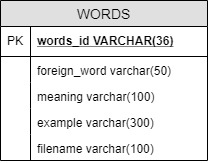
\includegraphics[width=.5\linewidth]{images/entity.jpg}
  \centering
  \caption{Adatbázis struktúra}
  \label{fig:entity}
\end{figure}

Ahhoz, hogy az alkalmazás további funkcióit, beleértve a pdf fájl, illetve tudásellenőrző teszt generálását implementálni tudjuk szükségünk van egy adatbázisra, amely az eddig elvégzett fordításokat tartalmazza kiegészítő adatokkal. Ehhez egy igazán könnyűsúlyú, egyszerűen telepíthető és használható adatbázist, a \textit{H2} adatbázist vettem segítségül. Használatához csupán a megfelelő függőséget kellett az alkalmazás \textit{.pom} állományába importálnom. Az adatbázist \textit{liquibase} segítségével hoztam létre. Az ehhez szükséges \textit{changelog.xml} mellett létrehoztam egy \textit{create-table.xml} fájlt, amely alapján a \textit{liquibase} megalkotja az adatbázistáblát, amely a \ref{fig:entity} számú ábrán látható. Ez a leírófájl 
úgynevezett \textit{changeSet}-eket tartalmaz, melyek adatbázis műveleteket írnak le, és a \textit{liquibase} sorban, egymás után hajt végre ezeket az adatbázison. Az első létrehozza a táblát, ha még az nem volt előtte létrehozva, a második pedig hozzáadja az elsődleges kulcsot, amely jelen esetben a \textit{words\_id}. Ez egy egyedi azonosító, melynek ismeretében pontosan meghatározható bármely rekord az adatbázisban. Formátuma \textit{UUID}, ami egy 36 karakter hosszú egyedi karakterlánc. A tábla további elemei:
\begin{itemize}
\item \textbf{ foreign\_word}, a mondatelem, amelyre a felhasználó kattintott, legfeljebb 50 karakter hosszú
\item \textbf{meaning}, a mondatelem jelentése(i), legfeljebb 100 karakter hosszú
\item \textbf{example}, példamondat, amely a mondatelem kontextusából kerül ki, legfeljebb 300 karakter hosszú
\item \textbf{filename}, feliratfájl neve, amelyben az aktuális mondatelem szerepelt, legfeljebb 100 karakter hosszú
\end{itemize}

Miután a tábla elkészült, lehetőség nyílik azon a szükséges adatbázis műveletek végrehajtására. Az objektumok a nyelvfordítás elvégeztével kerülnek be az adatbázisba. Amennyiben már megtalálhatóak ott, nem történik újbóli mentés. Mivel az alkalmazás működtetéséhez csupán néhány lekérdezésre, és beszúrásra volt szükségem, egyszerű \textit{jdbc} műveletek használata mellett döntöttem. Ezek a \textit{WordService} osztályban kerültek implementálásra. Megvalósított műveletek:
\begin{itemize}
\item \textbf{create}, a szavak adatbázisba történő mentésére szolgál
\item \textbf{getAllByFilename}, visszatér az összes szóval, melyek fájlnevei megegyeznek a paraméterben kapott fájlnévvel
\item \textbf{isAlreadySaved}, visszatérési értéke igaz vagy hamis, attól függően, hogy a paraméterben kapott szó megtalálható-e már az adatbázisban
\item \textbf{deleteAll}, törli az összes rekordot az adatbázisból
\item \textbf{getAll}, visszetér az összes adatbázisban található rekorddal
\end{itemize}
Egy metódus felépítése a következő: először létrehoz egy \textit{Connection} kapcsolatot, amely az adatbázisfájl, és a hozzá tartozó azonosítók (felhasználónév, jelszó) ismeretében lehetséges. Majd ezen végrehajt egy műveletet, melyet \textit{SQL} nyelven kell megadnunk a \textit{jdbc}-nek. Amennyiben a művelet végrehajtása közben kivétel dobódott, az alkalmazás egy \textit{JOptionPane} hibapanelt jelenít meg a képernyőn, a felhasználó tudtára adva, hogy váratlan hiba keletkezett a folyamat közben (\ref{lst:deleteAll}).

\begin{lstlisting}[caption=Implementált deleteAll metódus, language=java, label={lst:deleteAll}]
public void deleteAll() {
    try (Connection connection = DriverManager
    .getConnection("jdbc:h2:file:~/basicvlcj", "sa", "");
        Statement stat = connection.createStatement()) {
            stat.executeUpdate("DELETE FROM WORDS");
    } catch (SQLException e) {
        JOptionPane.showMessageDialog(JOptionPane.getRootFrame(),
        "An unexpected error has occurred",
        "Error",
        JOptionPane.ERROR_MESSAGE);
    }
}
\end{lstlisting}

Az imént említett függvények megvalósítása után egyszerűen lekérdezhetővé váltak a többi funkció által igényelt adatok. Így ezen komponensek implementálásával folytattam a fejlesztést.